\documentclass{standalone}
\usepackage{tikz}
\begin{document}
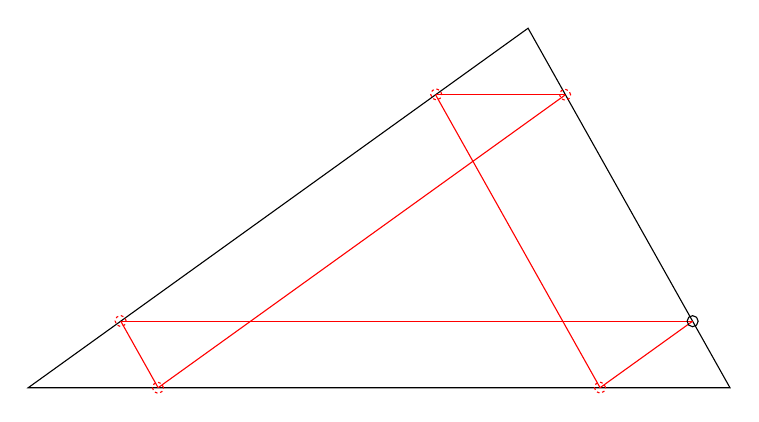
\begin{tikzpicture}[x=1pt,y=1pt]
\draw (15.99,-153.00) -- (269.56,-153.00) -- (196.61,-23.10) -- cycle;
\draw[red] (222.63,-153.00) -- (163.18,-47.14);
\draw[red] (163.18,-47.14) -- (210.12,-47.14);
\draw[red] (210.12,-47.14) -- (62.93,-153.00);
\draw[red] (62.93,-153.00) -- (49.43,-128.96);
\draw[red] (256.07,-128.96) -- (222.63,-153.00);
\draw[red] (49.43,-128.96) -- (256.07,-128.96);
\draw (256.07,-128.96) circle (2.00);
\draw[red, dash pattern=on 1pt] (222.59,-152.96) circle (2.00);
\draw[red, dash pattern=on 1pt] (163.44,-47.02) circle (2.00);
\draw[red, dash pattern=on 1pt] (209.99,-47.14) circle (2.00);
\draw[red, dash pattern=on 1pt] (49.39,-128.90) circle (2.00);
\draw[red, dash pattern=on 1pt] (62.86,-153.02) circle (2.00);
\end{tikzpicture}
\end{document}
